% -*- coding: utf-8 -*-
\documentclass[11pt]{oblivoir}
\usepackage[utf8]{inputenc}
\usepackage{kotex}
\usepackage[scale=0.75, twoside, bindingoffset=5mm, a4paper]{geometry}
\usepackage{indentfirst}
\usepackage{graphicx}
\usepackage{color}
\usepackage{pgf-pie}

\newenvironment{textbox}
	{
	\begin{center}
		\begin{tabular}{|p{0.95\textwidth}|}
			\hline
	}
	{
		\\ \hline
		\end{tabular}
		\end{center}
	}

\title{\textbf{엔씨소프트 분석을 통한 효율적인 경영 방법 및 비전 고찰}}
\author{\textbf{1학년 9반 15번 박태원}}

\begin{document}
	
	\begin{center}
		\maketitle
		\begin{abstract}
			논문 요약쓰		
		\end{abstract}
		\tableofcontents
		\pagebreak
	\end{center}


	\section{서론}
		\subsection{배경 및 선정 동기}
			\textbf{게임 엔터테인먼트 산업}은 4차 산업혁명의 역풍에 굴하지 않고 꾸준히 각광받고 있는 산업이다. 이에 국내 시장에서는 2015년 최초로 \textbf{10조원}이상의 매출액을 기록한 이후, `16년에는 \textbf{11조원}, `17년에는 \textbf{12조원}, 가장 최근인 `18년에는 \textbf{13조원}을 기록하며 지속적인 성장세를 보여주고 있다.\footnote{콘텐츠산업 2018년 결산 및 2019년 전망 보고서 34p}
			
			\begin{figure}[htbp]
				\centering
				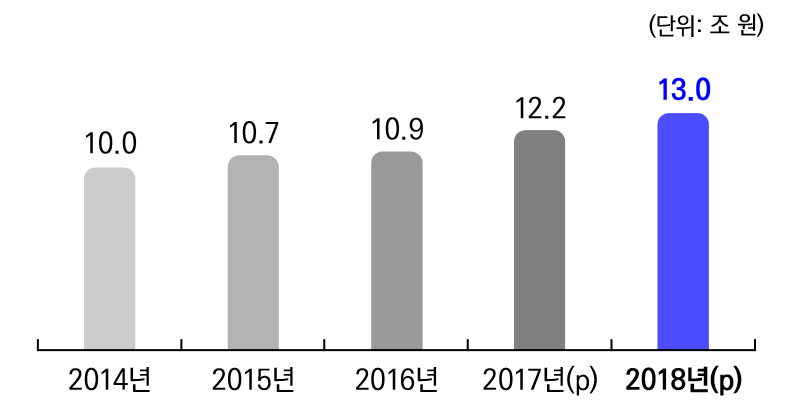
\includegraphics[width=1\textwidth]{GameMaechul.png}
				\caption{게임 산업 매출액 추이}
			\end{figure}
			
			또한 최근에는 \textbf{E-SPORTS 산업}의 성장으로 인해 \textbf{2020년까지 꾸준히 상승}할 것으로 전망되었다.\footnote{한국콘텐츠진흥원 대한민국 게임백서 2018 6p} 
			따라서 앞으로의 전망을 고려하였을 때, 게임 산업에 대하여 연구하는 것이 가치가 있을 것이라 판단하게 되었다.
			
			그 중에서도 이번 연구 대상이 된 기업인 \textbf{"엔씨소프트"}는 국내에서 오랜 세월 명목을 이어오고 있는 게임 개발사 중 하나이며, 한 때 온라인 게임계에 이름을 휘날렸던 \textbf{"아이온"}과 대한민국 게임계에 한 획을 그었다고 평가받는 \textbf{"리니지"} 시리즈를 개발하여 대한민국 게임 시장에 지대한 영향을 미치고 있는 기업이기도 하다. 
			
			이에 대한 통계로, 게임 퍼블리셔를 기준으로 정렬한 \textbf{2019년 상반기 모바일 게임 매출 점유율}을 들 수 있다. 다음은 그것을 도식화 한 것이다
			\footnote{MOBILEINDEX 2019년도 상반기 한국 모바일 게임 시장 총정리}
			
			\begin{figure}[htbp]
				\centering
				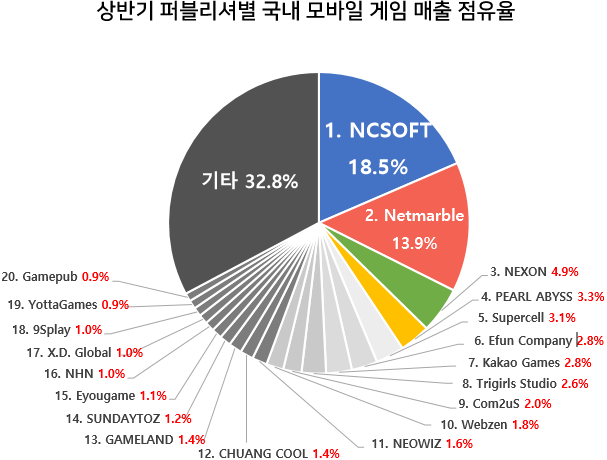
\includegraphics[width=1\textwidth]{MobileMaechul.png}
				\caption{2019년도 상반기 모바일 게임 매출 점유율 (퍼블리셔별)}
			\end{figure}
			
			이러한 관점에서 엔씨소프트가 \textbf{게임 엔터테인먼트 기업}의 표본으로서 적절한 뿐 만 아니라, 그 경영 전략을 분석하고 연구하기에도 상당히 가치있는 기업이라 판단하게 되었다. 
			
		\subsection{절차}
			선행 조사는 다음과 같은 절차로 진행한다.
			\begin{textbox}
				\textbf{1. 개요 조사} - 분석에 앞서, 기업에 대한 기본적인 이해를 위해 전반적인 개요에 대하여 조사한다.
				\\
				\textbf{2. 연혁 조사} - 기업 분석의 원활한 진행을 위하여, 앞서 기업의 연혁에 대하여 조사한다.
				\\
				\textbf{3. 비전 조사} - 기업의 비전이 전체 경영에 끼친 영향을 알아보기 위하여 이를 조사한다.
			\end{textbox}
			본론인 분석은 다음과 같은 절차로 진행한다.
			\begin{textbox}
				\textbf{1. 시장 분석} - 게임 시장의 전반적인 추세가 기업에 미친 영향을 분석한다.
				\\
				\textbf{2. 환경 분석} - SWOT 분석을 활용하여 주변 환경이 기업에 미친 영향을 분석한다.
				\\ 
				\textbf{3. 경쟁사 분석} - 경쟁사의 최근 횡보가 기업에 미친 영향에 대하여 분석한다.
				\\
				\textbf{4. 마케팅 분석} - 마케팅이 기업에 미친 전반적 영향에 대하여 분석한다.
				\\
				\textbf{5. 재무 분석} - 재무제표를 활용하여 재무상태 조사 및 그 원인을 분석한다.
				\\
				\textbf{6. 주가 분석} - 차트 및 뉴스를 통하여 기업의 주가에 영향을 끼친 원인을 분석한다.
			\end{textbox}
			결론은 주어졌던 연구 목적을 맺으며 끝낸다.
			\begin{textbox}
				\textbf{1. 기업 전망} - 본론에서 진행한 분석을 기반으로 예측되는 기업의 전망에 대해서 결론한다.
				\\
				\textbf{2. 내가 CEO라면} - 내가 CEO 였다면 어떤 전략과 비전을 내세운 경영을 할 것인지 고찰해본다. 
			\end{textbox}
	
	\section{선행 조사}
		\subsection{기업 개요}
		\noindent 엔씨소프트는 자사에 대해서 다음과 같이 소개하고 있다. 소개의 일부분을 인용하였다:
		
		\begin{textbox}
			엔씨소프트는 세계 최고의 개발 기술력과 서비스 역량을 보유한 온라인 게임 리더입니다.
			
			1997년, 엔씨소프트는 리니지를 시작으로 인터넷 기반 온라인 게임의 대중화를 이끌었으며, 해외 시장을 개척, 아시아, 북미, 유럽 등에 글로벌 네트워크를 확보해 나가고 있습니다.
		\end{textbox} 
		\pagebreak
		
		\noindent 또한 다음은 엔씨소프트에서 공개하고 있는 자사의 공식적인 정보다:
		\begin{enumerate}
			\item \textbf{회사명 :} (주)엔씨소프트
			\item \textbf{설립일 :} 1997년 3월
  			\item \textbf{대표이사 :} 김택진
			\item \textbf{등록 :} 2000년 7월 7일 코스닥 등록 
			\item \textbf{상장 :} 2003년 5월 22일 거래소 이전 상장
			\item \textbf{자본금 :} 약 100 억 원
		\end{enumerate}
		
		\subsection{기업 연혁}
			\noindent
			
			다음은 경영 실적에 영향을 미칠만한 연혁들을 정리한 것이다:
			\begin{textbox}
			\textbf{\textcolor{blue}{1997. 3}} 엔씨소프트 창립
			\\
			\textbf{\textcolor{blue}{1998. 9}} 게임  \textbf{리니지} 상용서비스 개시
			\\
			\textbf{\textcolor{blue}{2000. 5}} 글로벌 네트워크 구축개시 (해외법인)
			\\
			\textbf{\textcolor{blue}{2000. 7}} 해외 서비스 개시 (리니지 대만 서비스 시작)
			\\
			\textbf{\textcolor{blue}{2000. 7}} 코스닥 등록(2003년 한국증권거래소로 이전 상장)
			\\
			\textbf{\textcolor{blue}{2003. 10}} 게임 \textbf{리니지2} 서비스 개시
			\\
			\textbf{\textcolor{blue}{2005. 4}} \textbf{길드워} 상용서비스 개시 (북미 / 유럽 시장)
			\\
			\textbf{\textcolor{blue}{2008. 5}} 엔씨소프트 R\&D(Research \& Development) 센터 완공
			\\
			\textbf{\textcolor{blue}{2008. 11}} 게임 \textbf{아이온} 서비스 개시
			\\
			\textbf{\textcolor{blue}{2009.}} 게임 \textbf{아이온} 글로벌 론칭
			\\
			\textbf{\textcolor{blue}{2012. 6}} 게임 \textbf{블레이드 \& 소울} 서비스 개시
			\\
			\textbf{\textcolor{blue}{2012. 8}} 게임 \textbf{길드워 2} 상용서비스 개시
			\\
			\textbf{\textcolor{blue}{2013. 8}} 판교 R\&D 센터 완공
			\\
			\textbf{\textcolor{blue}{2014. 6}} 게임 \textbf{와일드스타} 북미/유럽 상용서비스 개시
			\\
			\textbf{\textcolor{blue}{2015. 5}} 북미법인 엔씨웨스트(NC West)의 모바일 스튜디오 설립
			\\
			\textbf{\textcolor{blue}{2015. 10}} 게임 \textbf{길드워2: 가시의 심장} 상용서비스 개시
			\\
			\textbf{\textcolor{blue}{2016. 1}} 게임 \textbf{블레이드 \& 소울} 북미/유럽 정식 서비스 돌입
			\\
			\textbf{\textcolor{blue}{2016. 12}} 게임 \textbf{리니지 레드나이츠} 아시아 12개국 정식 서비스
			\\
			\textbf{\textcolor{blue}{2017. 6}} 게임 \textbf{리니지 M} 서비스 개시
			\\
			\textbf{\textcolor{blue}{2017. 6}} 게임 \textbf{MXM} 북미/유럽 출시
		\end{textbox}
		\subsection{기업 비전}
		
		\subsubsection{기업 CI}
			
\includegraphics[width=1\textwidth]{ci.png}
	\section{본론}
		\subsection{시장 분석}
		
		\subsection{환경 분석}
		
		\subsection{경쟁사 분석}
		
		\subsection{마케팅 분석}
		
		\subsection{재무 분석}
		
		\subsection{주가 분석}
	
	\section{결론}
	
	\section{레퍼런스}
	

\end{document}